\section{Anàlisis de les dades}
En aquest treball hi ha un conjunt de dades de vint mil mostres sobre el reconeixement de lletres en una caixa rectangular. La naturalesa de les variables són numèriques i són nombres enters, les variables són factors al reconèixer la lletra com per exemple, valor horitzontal i vertical a la caixa, mitjana de píxels a la caixa, variància.

\begin{verbatim}
       V2               V3               V4               V5               V6        
 Min.   : 0.000   Min.   : 0.000   Min.   : 0.000   Min.   : 0.000   Min.   : 0.000  
 1st Qu.: 3.000   1st Qu.: 5.000   1st Qu.: 4.000   1st Qu.: 4.000   1st Qu.: 2.000  
 Median : 4.000   Median : 7.000   Median : 5.000   Median : 6.000   Median : 3.000  
 Mean   : 4.024   Mean   : 7.035   Mean   : 5.122   Mean   : 5.372   Mean   : 3.506  
 3rd Qu.: 5.000   3rd Qu.: 9.000   3rd Qu.: 6.000   3rd Qu.: 7.000   3rd Qu.: 5.000  
 Max.   :15.000   Max.   :15.000   Max.   :15.000   Max.   :15.000   Max.   :15.000
 
       V7               V8             V9              V10              V11        
 Min.   : 0.000   Min.   : 0.0   Min.   : 0.000   Min.   : 0.000   Min.   : 0.000  
 1st Qu.: 6.000   1st Qu.: 6.0   1st Qu.: 3.000   1st Qu.: 4.000   1st Qu.: 7.000  
 Median : 7.000   Median : 7.0   Median : 4.000   Median : 5.000   Median : 8.000  
 Mean   : 6.898   Mean   : 7.5   Mean   : 4.629   Mean   : 5.179   Mean   : 8.282  
 3rd Qu.: 8.000   3rd Qu.: 9.0   3rd Qu.: 6.000   3rd Qu.: 7.000   3rd Qu.:10.000  
 Max.   :15.000   Max.   :15.0   Max.   :15.000   Max.   :15.000   Max.   :15.000
 
       V12              V13              V14              V15              V16           
 Min.   : 0.000   Min.   : 0.000   Min.   : 0.000   Min.   : 0.000   Min.   : 0.000   
 1st Qu.: 5.000   1st Qu.: 7.000   1st Qu.: 1.000   1st Qu.: 8.000   1st Qu.: 2.000   
 Median : 6.000   Median : 8.000   Median : 3.000   Median : 8.000   Median : 3.000   
 Mean   : 6.454   Mean   : 7.929   Mean   : 3.046   Mean   : 8.339   Mean   : 3.692   
 3rd Qu.: 8.000   3rd Qu.: 9.000   3rd Qu.: 4.000   3rd Qu.: 9.000   3rd Qu.: 5.000     
 Max.   :15.000   Max.   :15.000   Max.   :15.000   Max.   :15.000   Max.   :15.000   

      V17     
 Min.   : 0.000  
 1st Qu.: 7.000  
 Median : 8.000  
 Mean   : 7.801  
 3rd Qu.: 9.000
 Max.   :15.000
\end{verbatim}

Les variables són:
\begin{description} 
  \item[$\bullet$ V1-lettr:]  lletra majuscula
  \item[$\bullet$ V2-xbox:]  posició horitzontal de la caixa
  \item[$\bullet$ V3-ybox:]  posició vertical de la caixa
  \item[$\bullet$ V4 width:]  ample de la caixa
  \item[$\bullet$ V5-high:]  altura de la caixa
  \item[$\bullet$ v6-onpix:]  nombre total de píxels
  \item[$\bullet$ v7-xbar:]  mitjana x dels píxels de la caixa
  \item[$\bullet$ v8-ybar: ] mitjana y dels píxels de la caixa
  \item[$\bullet$ v9-x2bar] mitjana de la variancia de x 
  \item[$\bullet$ v10-y2bar] mitjana de la variancia de y
  \item[$\bullet$ v11-xybar] mitjana de la correlació x i y
  \item[$\bullet$ v12-x2ybr] mitjana de *x i *y
  \item[$\bullet$ v13-xy2br] mitjana de x * y* y
  \item[$\bullet$ v14-xege]  mitjana del número d'arestes d'esquerra a dreta
  \item[$\bullet$ v15-xegvy] correlació de x-ege amb y
  \item[$\bullet$ v16-yege] mitjana del número d'arestes de baix a adalt.
  \item[$\bullet$ v17-yegvx] correlació de y-ege amb x 
\end{description}

En analitzar les dades es veu que tots el valors de les variables van entre 0 i 15, que no hi han valors faltants, com ve surt a la descripció del conjunt de dades, i a més a més fent un sumari de les dades es pot observar que efectivament tots els valors són entre 0 i 15 i no hi han valors anormals. A més la distribució de les lletres reconegudes és uniforme i, per tant, es pot dir que el conjunt de dades està ben distribuït en el nombre de mostres per cada lletra del alfabet.

\begin{figure}[H]
    \centering
    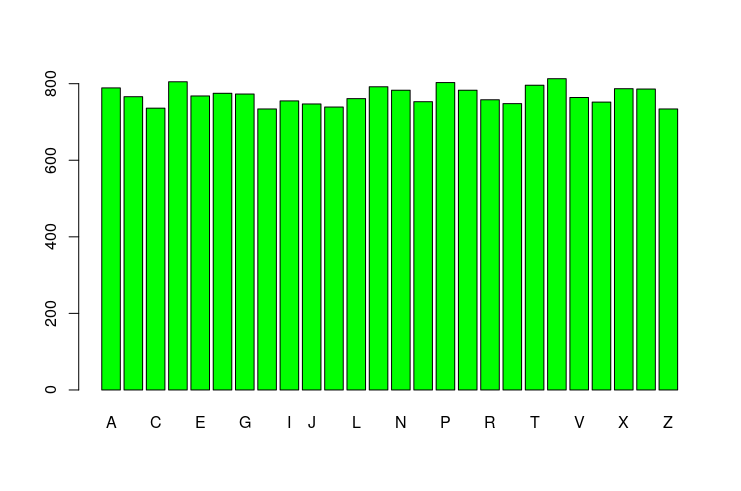
\includegraphics[width=10cm]{img/distribuciolletres.png}
    \caption{Distribució de les mostres en les lletres predites.}
    \label{fig:distrdataset}
\end{figure}

\section{Protocol de remostreig}\label{prepros}
Per tal de poder evaluar els diferents models de la manera més equitativa possible s'ha dividit el conjunt de dades en dos subconjunts d'entrenament i de prova. Per fer-ho s'ha dividit el conjunt original mantenint la proporcionalitat de la variable V1 (lletra de l'alfabet que es reconeix) utilitzant un 70\% de les mostres per al subconjunt de entrenament i el 30\% restant pel subconjunt de prova. Per a tots els models s'utilitzen els mateixos conjunts per entrenar i provar per tal de mantenir la coherència.

Per tal d'ajustar els paràmetres òptims de cada model sense caure en un sobreajust, hem fet servir \textit{Cross-Validation}, per a cada model hem utilitzat una variant de \textit{Cross-Validation} que s'ajustés millor, per exemple per a models més complexes hem utilitzat \textit{5-fold Cross-Validation} i en models més simples \textit{10-fold Cross Validation} per ajustar el temps d'execució. Altrament, en altres hem utilitzat \textit{Leave-One-Out Cross-Validation}. Per utilitzar \textit{Cross-Validation} utilitzem la llibreria de R \textit{caret}.
\cite{caretlibrary}

Durant la resta del treball prendrem com a mesura de l'error i de precisió com les respectives fórmules:
\[\text{error} = 1 -(\frac{\text{observacions correctes}}{\text{observacions totals}})\]
\[\text{precisió} = (\frac{\text{observacions correctes}}{\text{observacions totals}})\]
